 \section{Build instructions}
    The contents of submission is as follows:
    
    |- SUBMISSION\_ROOT \\
    |\quad|- cxx \\
    |\quad\quad |- src \\
    |\quad\quad\quad |- common \# Definition of classes, tool functions\\ 
    |\quad\quad\quad |- tcpClient \# TCP client implementation (C/S)\\
    |\quad\quad\quad |- tcpNode \# TCP node implementation (P2P)\\
    |\quad\quad\quad |- tcpServer \# TCP server implementation (C/S)\\
    |\quad\quad\quad |- tcpTracker \# TCP tracker implementation (P2P) \\
    |\quad\quad -- CMakeLists.txt \\
    |\quad-- mininet\_run.py \# Minet experiment\\

\subsection{Requirement}
\begin {itemize}
\item Linux Operating System (Ubuntu 18.04 LTS tested)
\item CMake
\item Clang that support C++11 standard
\item Python3
\item Mininet
\end {itemize}

\subsection{Build CXX executables}
Run the following script to build CXX executables:
\begin{lstlisting}[language=bash]
cd $SUBMISSION_ROOT
mkdir build
cd build && cmake ../cxx && make
\end{lstlisting}
The executables are generated in the $\mathtt{build}$ directory

\subsection{Usage of CXX executables}
\subsubsection{Usage of tcpServer and tcpClient}
The  $\mathtt{tcpServer}$ is launched this way:
\begin{lstlisting}[language=bash]
./tcpServer [Root path]
\end{lstlisting}
The  $\mathtt{tcpClient}$ is launched this way:
\begin{lstlisting}[language=bash]
./tcpClient [Host IP] [Host Port] [FILEPATH (Remote)] [FILEPATH (Local)]
\end{lstlisting}
or this way:
\begin{lstlisting}[language=bash]
./tcpClient
\end{lstlisting}
$\mathtt{FILEPATH (Remote)}$ refers to the desired file's path on the server side. The path is relative to the server's $\mathtt{Root path}$.$\mathtt{FILEPATH (Local)}$ refers to the local path where the file will be saved (must exist).

If no argument were passed to $\mathtt{tcpClient}$, a command line interface will be started. The program will wait for input. It expect the user to provide the IP and port where a $\mathtt{tcpServer}$ is running. Then it connects to the server and list its directories. User can use following commands to interact with it:
\begin{itemize}
\setlength{\itemsep}{0pt}
\item[-] cd [Dir]           \# Change directory
\item[-] ls                    \# List directory
\item[-] dl  [Filename] \# Download file
\end{itemize}

\subsubsection{Usage of tcpServer and tcpClient}
The  $\mathtt{tcpTracker}$ is launched this way:
\begin{lstlisting}[language=bash]
./tcpTracker 
\end{lstlisting} 
The tracker listen to peers requests. It must be launched before $\mathtt{tcpNode}$

The  $\mathtt{tcpNode}$ is launched this way:
\begin{lstlisting}[language=bash]
./tcpNode [PORTDelta] [TRACKERHOSTNAME] [TRACKERPORT] [ROOTPATH] [FILE1] [FILE2] 
\end{lstlisting} 

$\mathtt{PORTDelta}$ represent the offset of Node's listen port from $\mathtt{NODEPORT}$ defined in $\mathtt{macro.h}$, this is designed to better debug the program on single host. $\mathtt{TRACKERHOSTNAME} $ and $\mathtt{RACKERPORT}$ are IP and port where $\mathtt{tcpTracker}$ listen. $\mathtt{ROOTPATH}$ is the the root path of Node. $\mathtt{FILE*}$ are filenames separated by spaces, referring to the files the user want to sync

The tcpNodes can be launched at any sequence, but if none of the tcpNodes have desired file, nothing will be transmitted.

\subsection{Usage of Python script}
To run the experiment, simply execute
\begin{lstlisting}[language=bash]
sudo python3 mininet_run.py
\end{lstlisting} 
or
\begin{lstlisting}[language=bash]
sudo python3 mininet_run.py --max_client 5 --min_client 2 --fs 10 --delay 3 --bw 10
\end{lstlisting} 
The default value of max/min number of client is 5 and 1. The default value of the file size is 10MiB. 

There are 7 stages: 
\begin{itemize}
\setlength{\itemsep}{0pt}
\item 1) The script build CXX executable. 
\item 2) The script delete possible old experiment output 
\item 3) The script prepare test folders, generate random download/sync target.
\item 4) The script create Mininet topology.
\item 5) The script run tests, redirect standard output to log files and wait enough time.
\item 6) The script checks file integrity by running $\mathtt{md5sum}$
\item 7) The script read log files and plot results
\end{itemize}

A formula was used to estimate how long the script should wait before all client/node have finished their work:
$$ t = \frac{3 \times 8 \times F \times (N+1)}{B}$$
where $F$ refers to file size in MiB, $N$ refers to number of clients and $B$ refers to Bandwidth.

Sometimes, the C/S model will fail to deliver file even under this time limit. In this case, a $\mathtt{md5sum}$ hash will detect this issue.

After the experiment, the file structure looks like:

    |- SUBMISSION\_ROOT \\
    |\quad|- build \\
    |\quad\quad-- tcpClient \\
    |\quad\quad-- tcpNode \\
    |\quad\quad-- tcpServer \\
    |\quad\quad-- tcpTracker \\
    |\quad\quad-- ... \\
    |\quad|- cxx \\
    |\quad|- Files \\
    |\quad\quad-- File\_XXM \\
    |\quad|- Dst \\
    |\quad\quad|- CS\\
    |\quad\quad\quad|- Downloads \\
    |\quad\quad\quad\quad-- Client1\_FileXXM\\
    |\quad\quad\quad\quad-- Client2\_FileXXM\\
    |\quad\quad\quad\quad-- ...\\
    |\quad\quad\quad-- Client1.log\\
    |\quad\quad\quad-- Client2.log\\
    |\quad\quad\quad-- ...\\
    |\quad\quad|- P2P\\
    |\quad\quad\quad|- Node1\\
    |\quad\quad\quad\quad-- File\_XXM\\
    |\quad\quad\quad|- Node2\\
    |\quad\quad\quad|- ...\\
    |\quad\quad\quad-- Node1.log\\
    |\quad\quad\quad-- Node2.log\\
    |\quad\quad\quad-- ...\\
    |\quad|- mininet\_run.py \\

    
Details are explained in script comments.
\section{Client/Sever model}
The structure of Client/Server model is shown in Figure \ref{cs}
\begin{figure}[H]
	\centering
	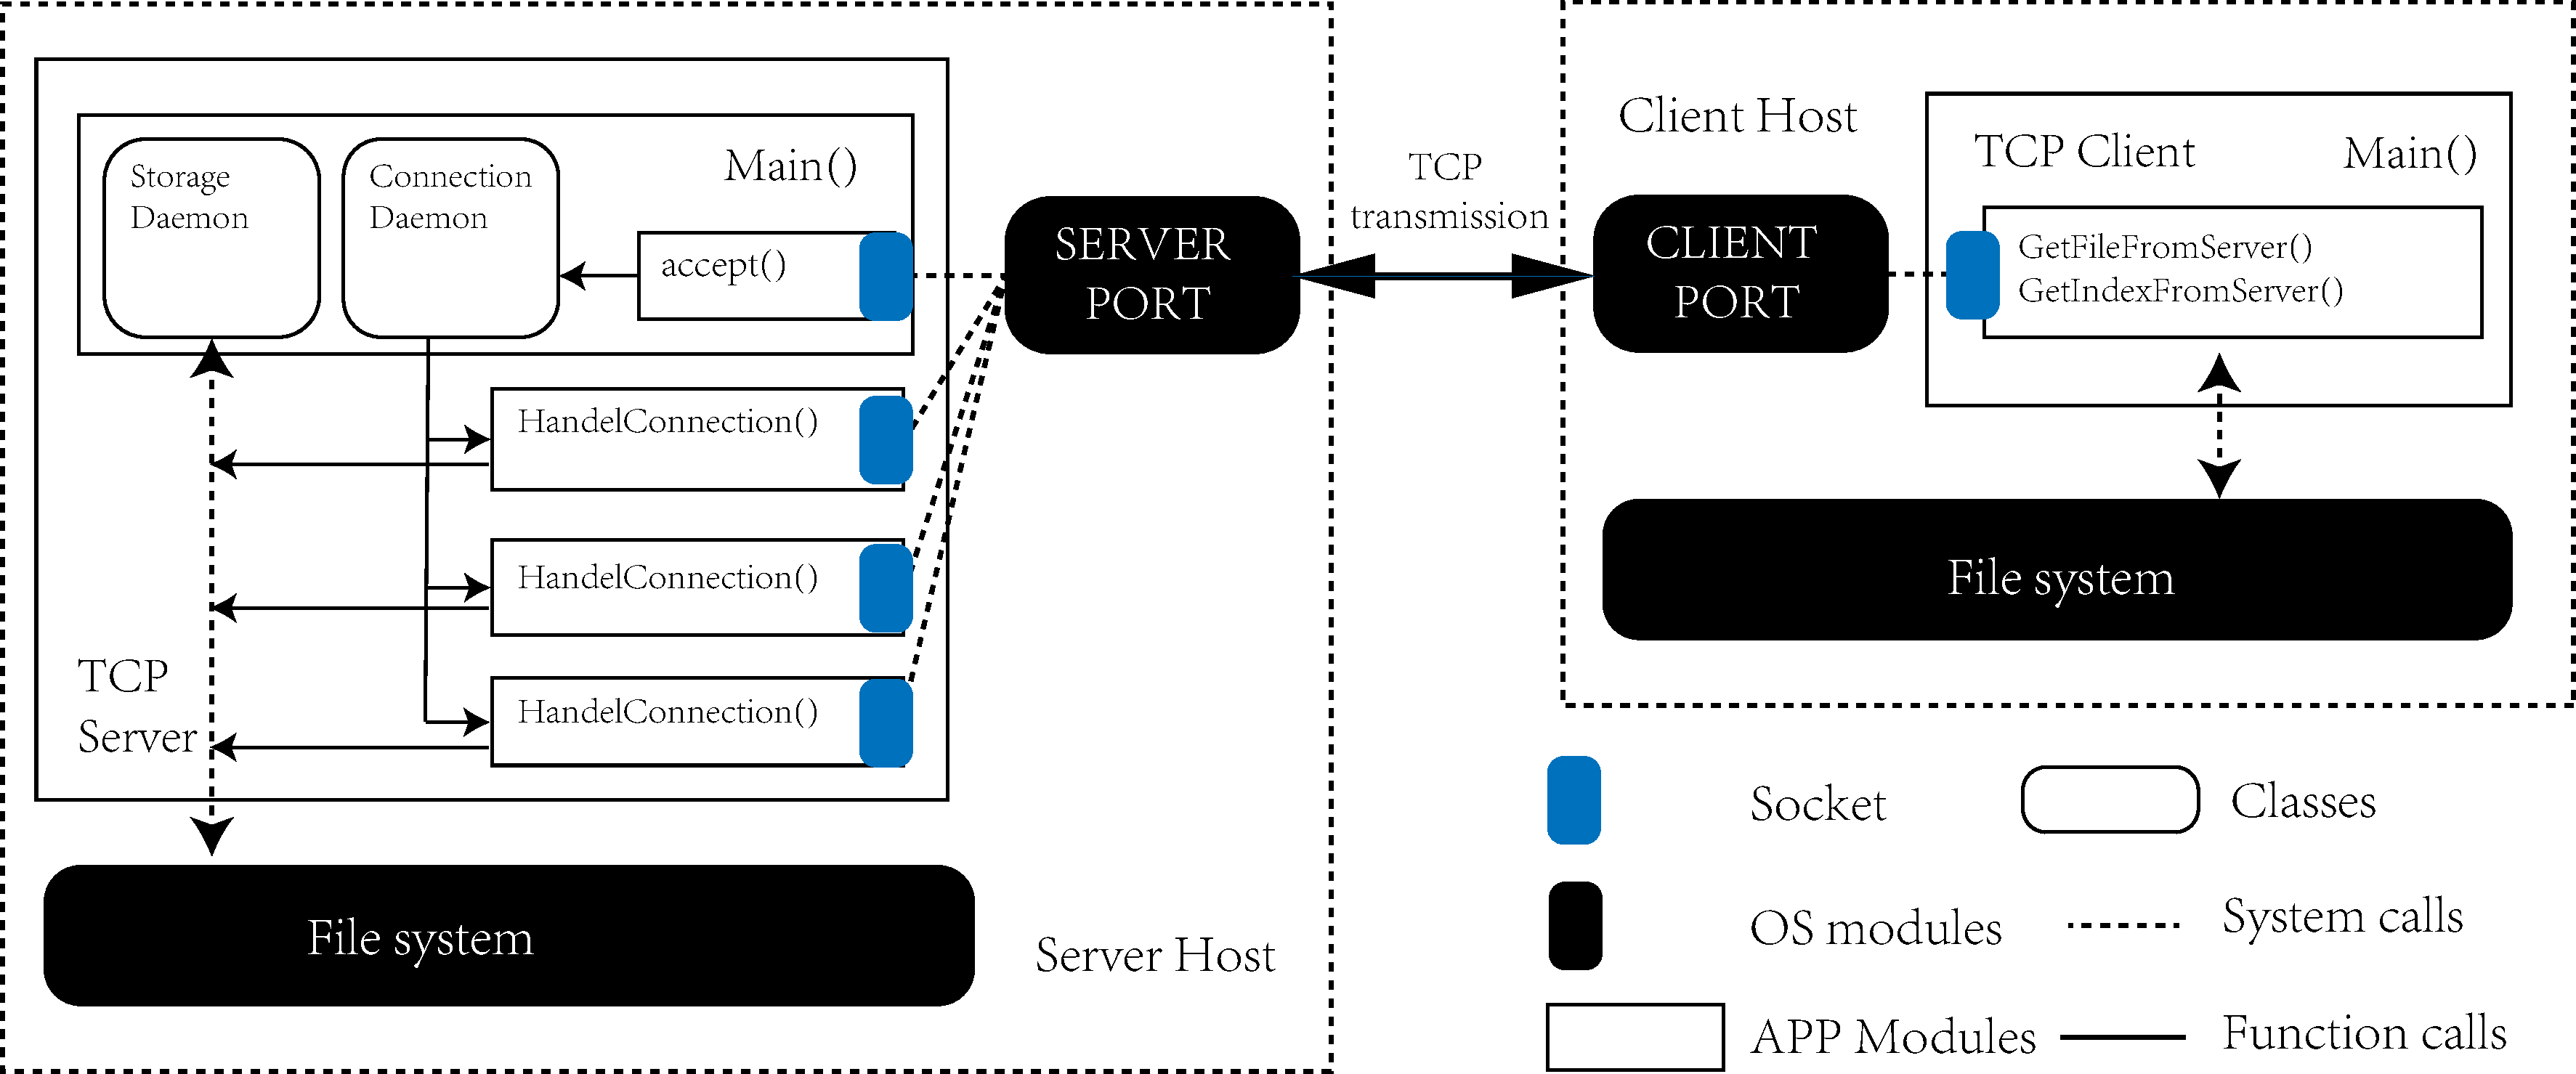
\includegraphics[scale=0.23]{img/cs}
	\caption{A structure design of C/S model}
	\label{cs}
\end{figure}
The server opens multiple threads for incoming clients. When sending a file, the server first send the size of the file, then send the file content in binary. 
The clients are single threaded. They talk to server by sending fixed-length strings (control messages). The length of these strings are defined in $\mathtt{macros.h}$.

\section{P2P model}
The structure of P2P model is shown in Figure \ref{p2p}
\begin{figure}[H]
	\centering
	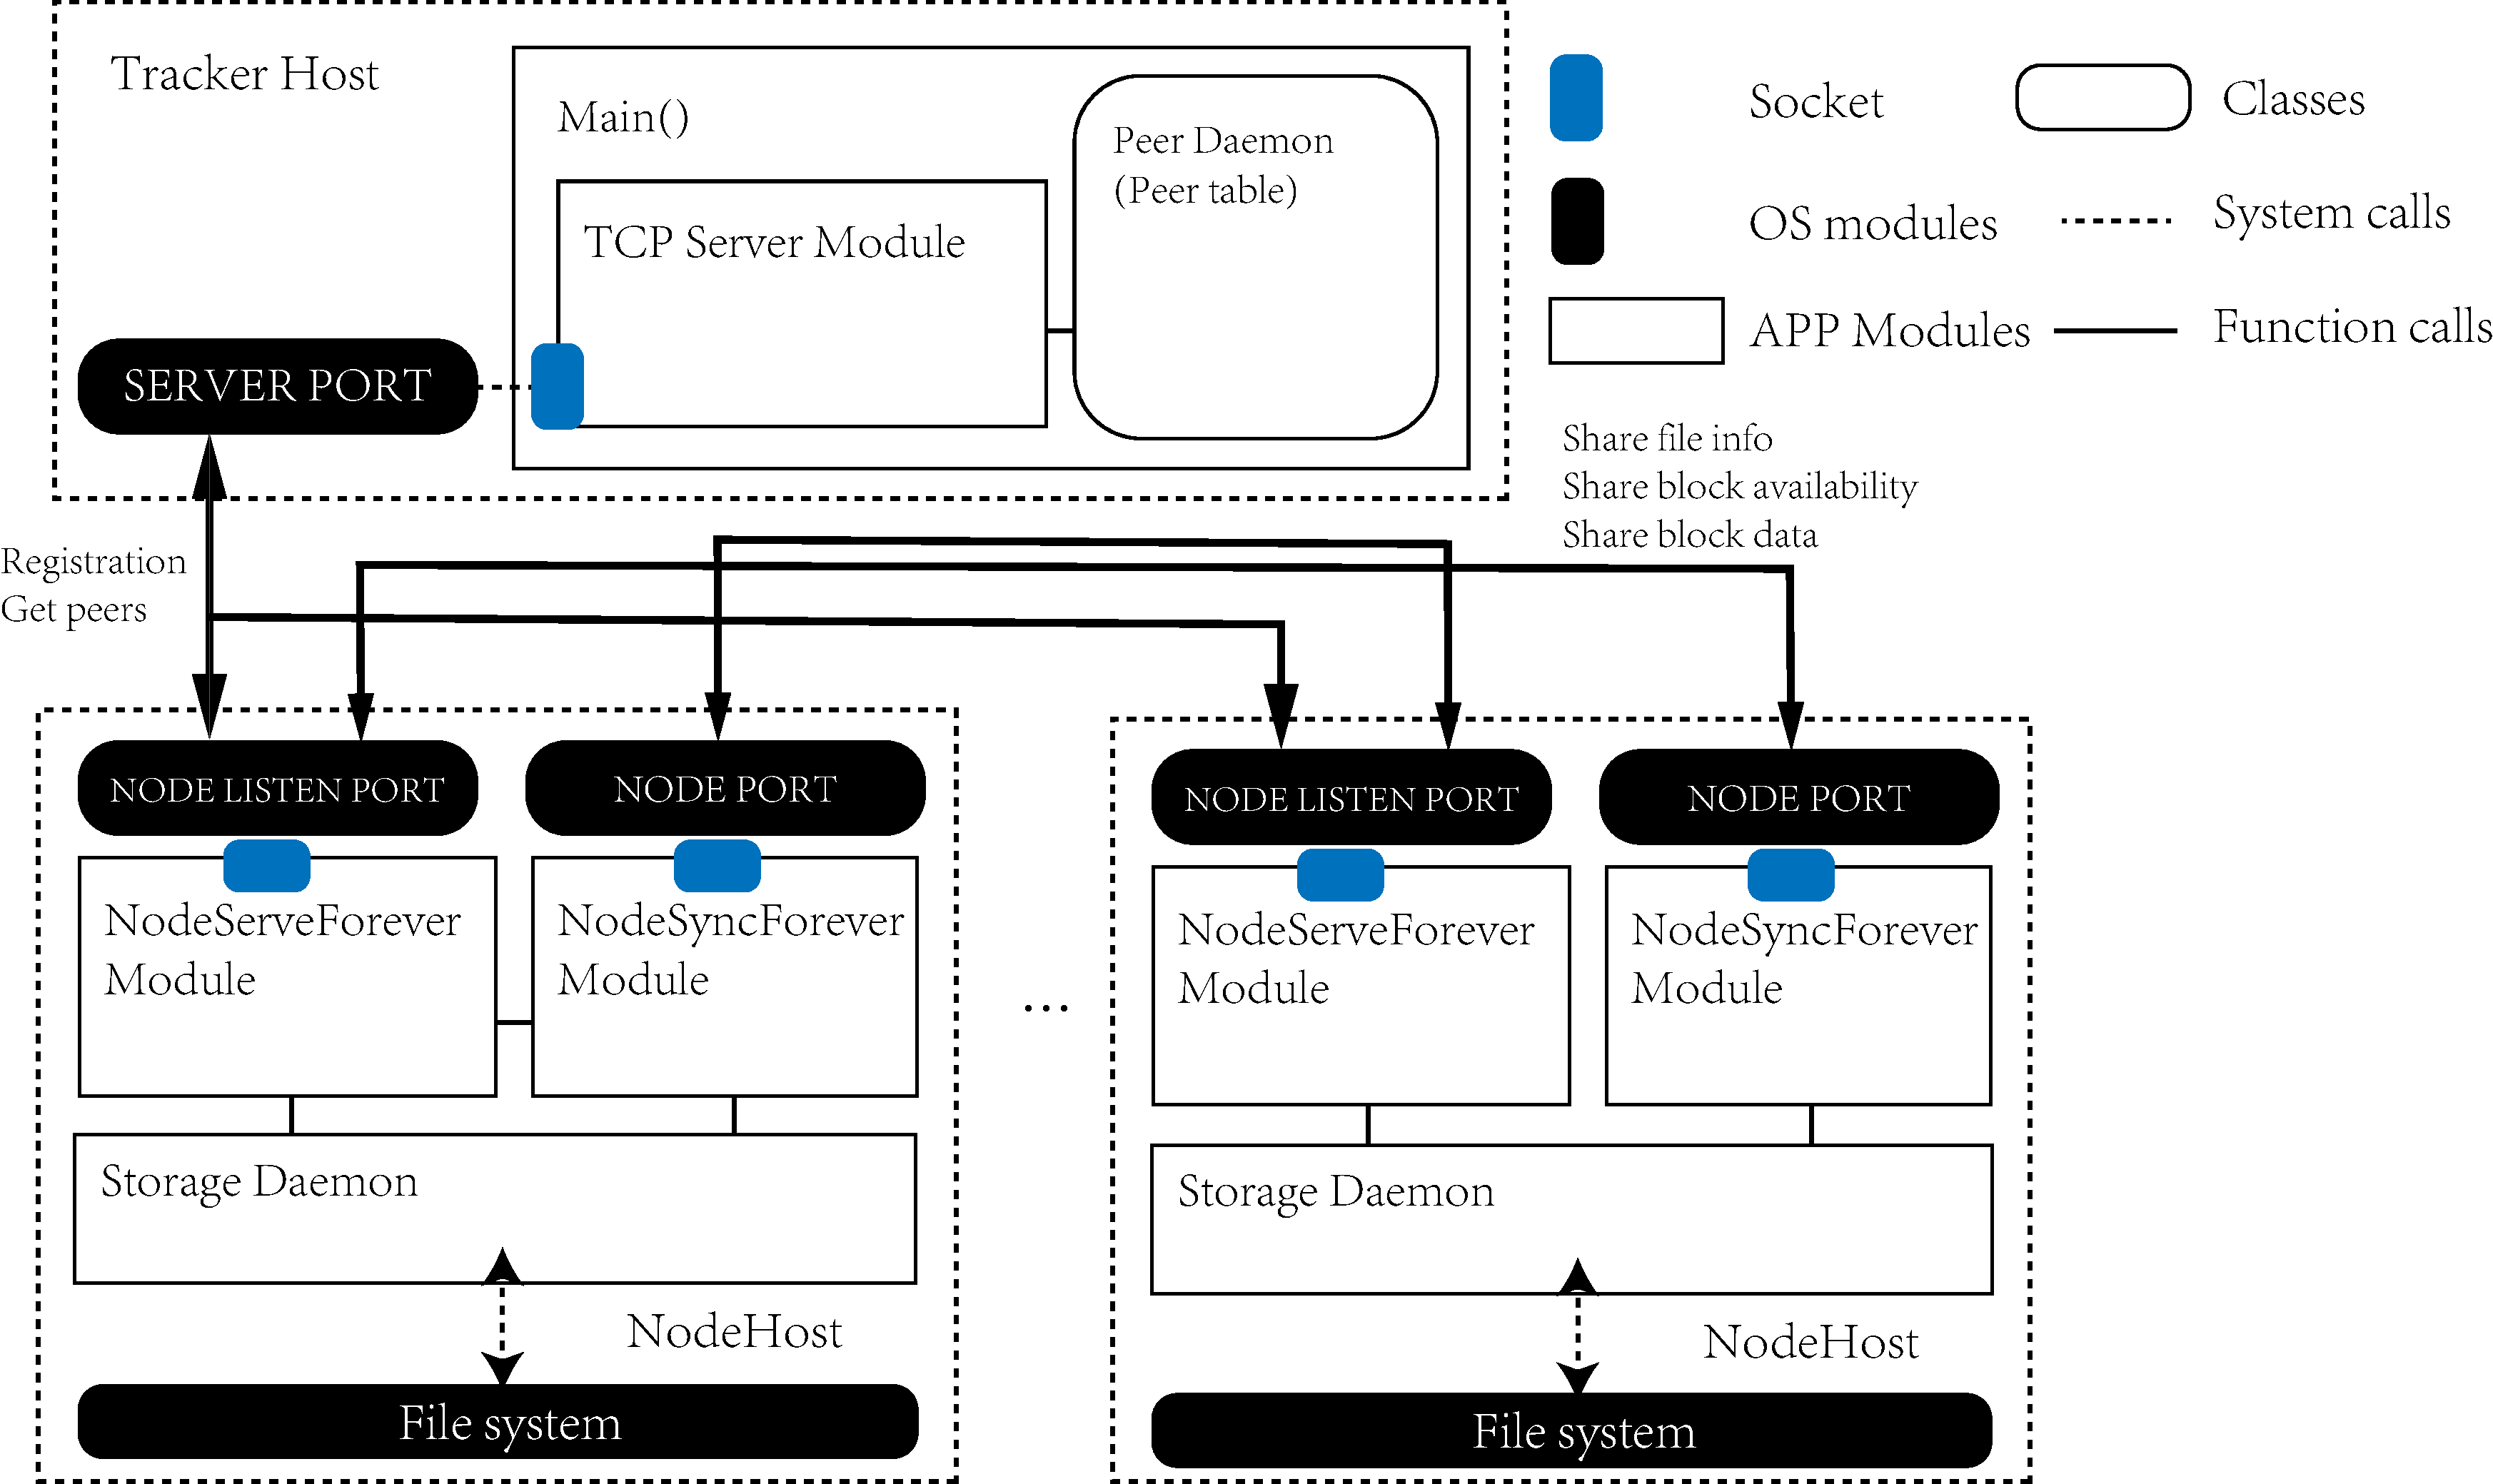
\includegraphics[scale=0.21]{img/p2p}
	\caption{A structure design of P2P model}
	\label{p2p}
\end{figure}
In our experiment, each node opens multiple threads for receiving and sending. The sending threads are managed in the same way as the $\mathtt{tcpServer}$. The receiving threads are synced by mutex.

The client get peer information from tracker. It also register itself to the tracker by multiplexing its listen port.
\section{Experiment}
We run the experiment. An example of standard output is shown in Figure \ref{screenshot}
\begin{figure}[H]
	\centering
	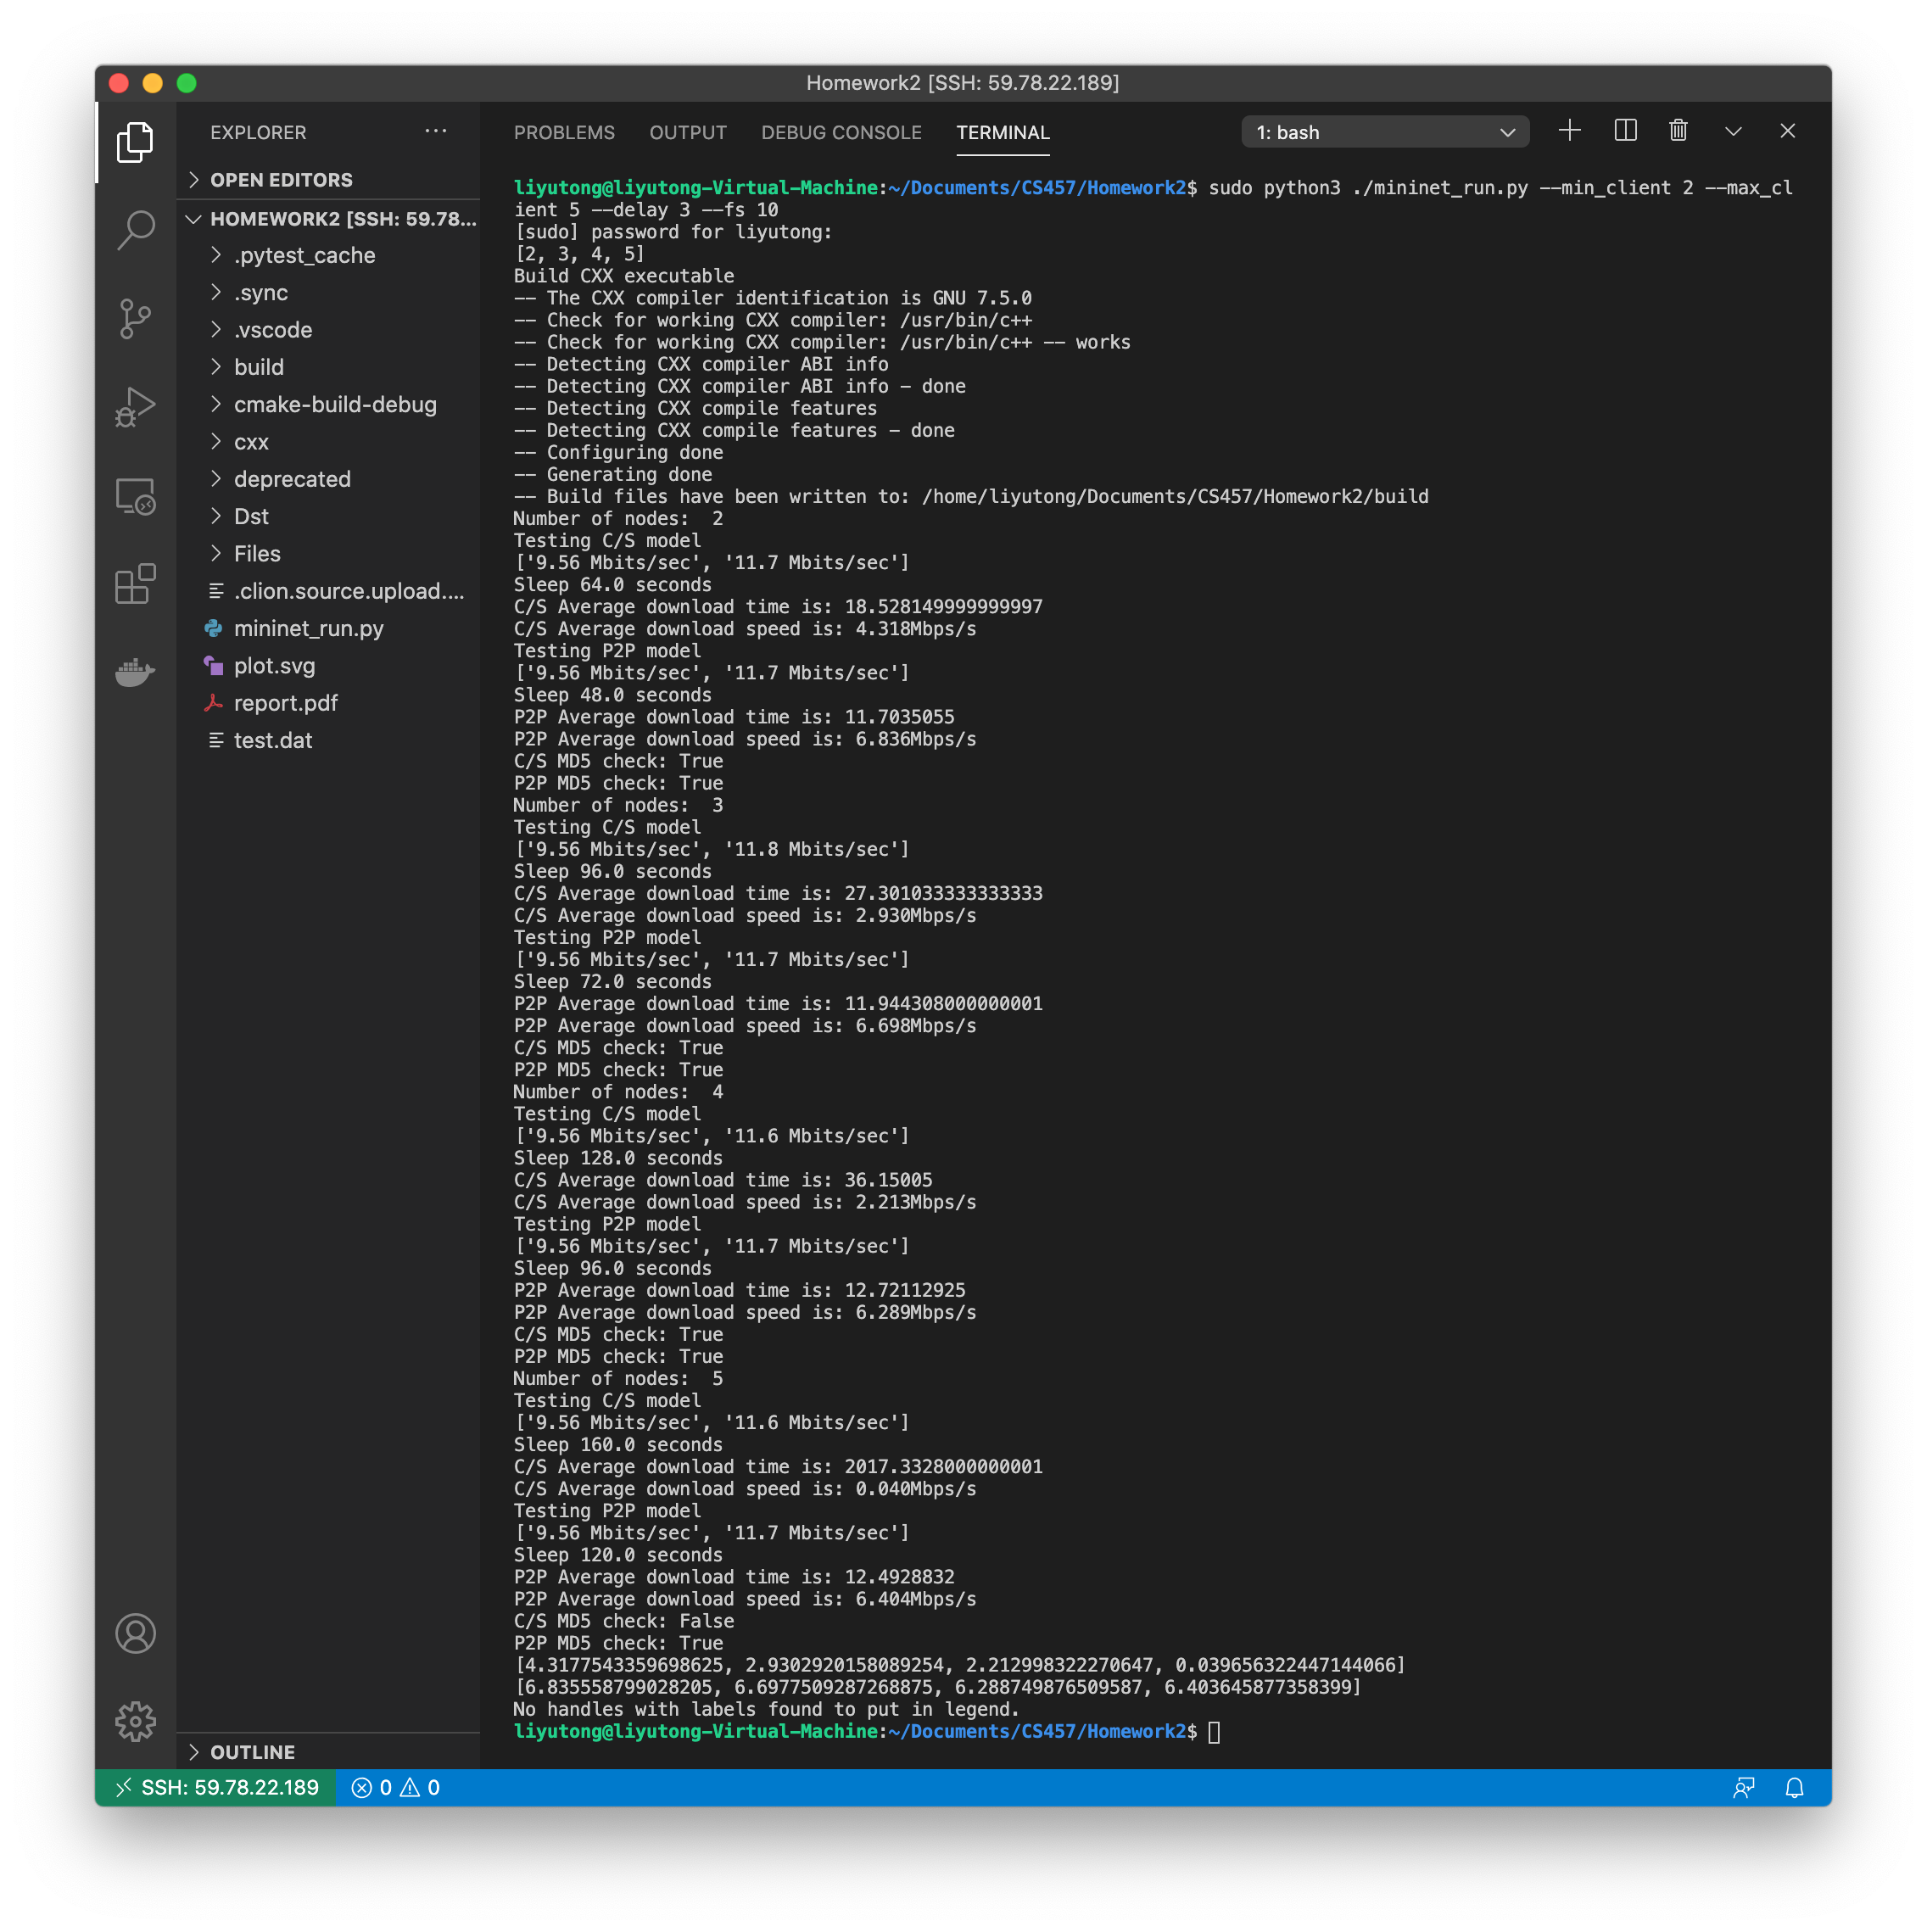
\includegraphics[scale=0.35]{img/run}
	\caption{Screenshot of standard output $\mathtt{Number \ Client} \in {2,3,4,5}$}
	\label{screenshot}
\end{figure}
\subsection{Iperf test}
We tested the connection speed between $\mathtt{Mininet}$ virtual hosts. The results are shown in Figure \ref{screenshot}


\subsection{C/S model (simutaneously)}
We launch the server, then launch a certain number of clients.

\begin{lstlisting}[language=python]
    hosts[0].cmd('./build/tcpServer ./Files/ > ./Dst/CS/Server.log&')
    for i in range(1, num_client + 1):
        hosts[i].cmd('./build/tcpClient 10.10.0.1 18889 ./File_{}M ./Dst/CS/Downloads/Client{}_File_{}M > ./Dst/CS/Client{}.log&'.format(file_size, i, file_size, i))
\end{lstlisting}

\subsection{P2P model (simutaneously)}
We launch the tracker, then launch a certain number of nodes immediately and simutaneously. The first node has the file.

\begin{lstlisting}[language=python]
    hosts[0].cmd('./build/tcpTracker > ./Dst/P2P/Tracker.log&')
    for i in range(1, num_client + 2):
        cmd_string = './build/tcpNode 0 10.10.0.1 18888 ./Dst/P2P/Node{}/ File_{}M  > ./Dst/P2P/Node{}.log&'.format(i, file_size, i)
        hosts[i].cmd(cmd_string)
\end{lstlisting}


\subsection{P2P model (in order)}
We launch the tracker, then launch a certain number of nodes in order. After each lauch, the script wait for 3 seconds.

\begin{lstlisting}[language=python]
    hosts[0].cmd('./build/tcpTracker > ./Dst/P2P/Tracker.log&')
    for i in range(1, num_client + 2):
        cmd_string = './build/tcpNode 0 10.10.0.1 18888 ./Dst/P2P/Node{}/ File_{}M  > ./Dst/P2P/Node{}.log&'.format(i, file_size, i)
        hosts[i].cmd(cmd_string)
        time.sleep(time_delay)
\end{lstlisting}


\section{Analyze of results}
\subsection{Simutaneous launch}
We carried out a set of experiment with number of peers ranging from 1 to 15. The result is shown in the Figure \ref{graph}
\begin{figure}[H]
	\centering
	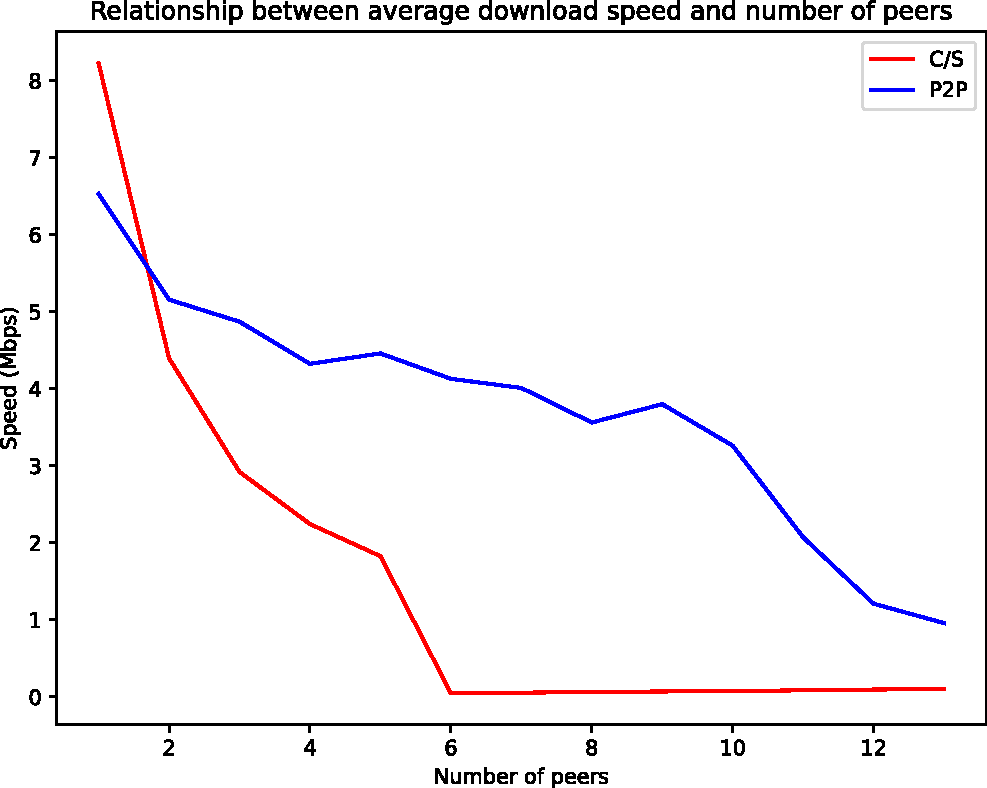
\includegraphics[scale=0.6]{img/graph}
	\caption{Relationship between average download speed and number of peers, file size = 10MiB}
	\label{graph}
\end{figure}
With a number of clients of 1, the P2P model is slightly slower than the C/S model because the client always tries to get more Peers from the tracker, and there are frequent exchanges between Peer and Peer about the latest state of the file, a transfer efficiency that could be improved if it had a more complex and refined control algorithm.

The average transmission rate of the network under the C/S model decreases substantially as the number of clients increases. According to the model, the decrease should be inversely proportional to the number of clients.The experimental data are roughly consistent with it.On the other hand, the average bandwidth of the network under the P2P model is significantly higher than the average speed under the C/S model.

As the number of clients continues to increase, the average speed of the network continues to decrease. A performance analysis revealed that the host CPU usage was close to 100\%. We speculate that the network cannot increase the transmission rate indefinitely due to the processing performance of the host. In addition, nodes under the P2P model require additional computation and communication, and have more disk read overhead, all of which result in a decrease in the average speed of the P2P network.

\subsection{Sequence launch}
In the P2P model, if clients are launched simutaneously, clients will try to receive blocks of file from their peers. At the beginning of the network, only on peer has the complete file. As a result, the peers are force to wait.


\begin{figure}[H]
	\centering
	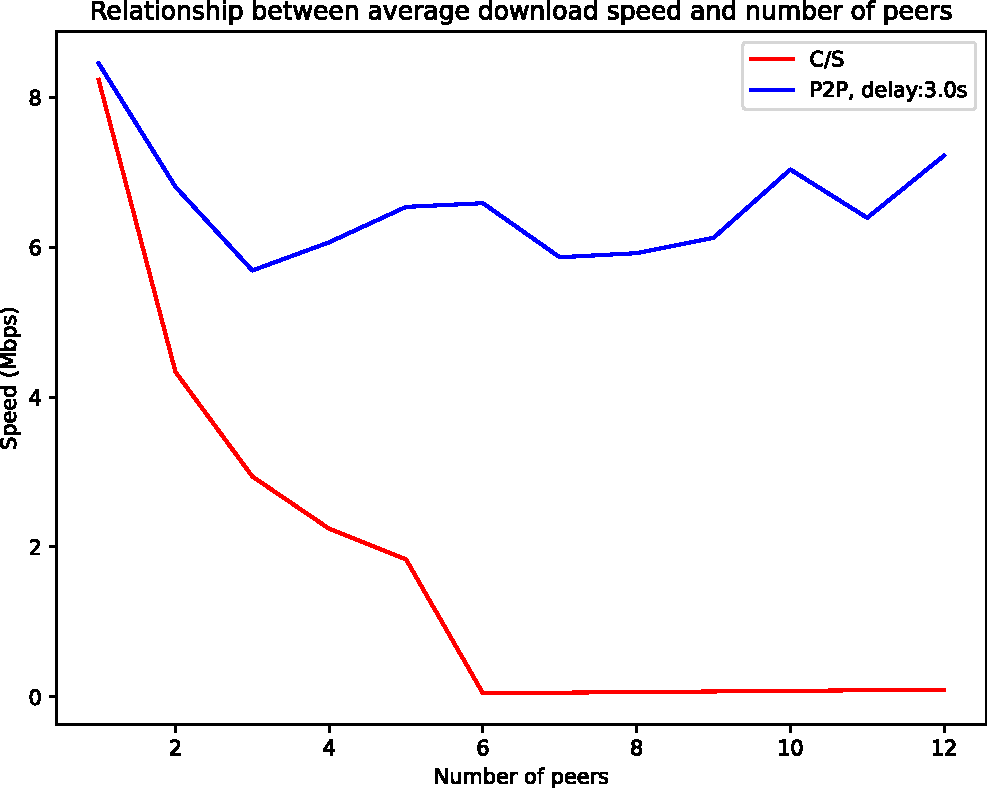
\includegraphics[scale=0.6]{img/graphdelay}
	\caption{Relationship between average download speed and number of peers, file size = 10MiB, delay=3s}
	\label{graphdelay}
\end{figure}

A solution is launching Nodes in a sequence. When we start the Nodes one by one, we can see that the average synchronization time across the network (the time it takes for a Node to complete synchronization) is reduced, resulting in an increase in the average download rate per node as shown in Figure \ref{graphdelay}. This is because later node gets the file block from its Peer immediately, which is in line with the P2P network transfer rules.

\subsection{The upload status of Node1}
In our experiment, Node1 is the peer who prossess the file initially. We are interested in its log
\begin{figure}[H]
	\centering
	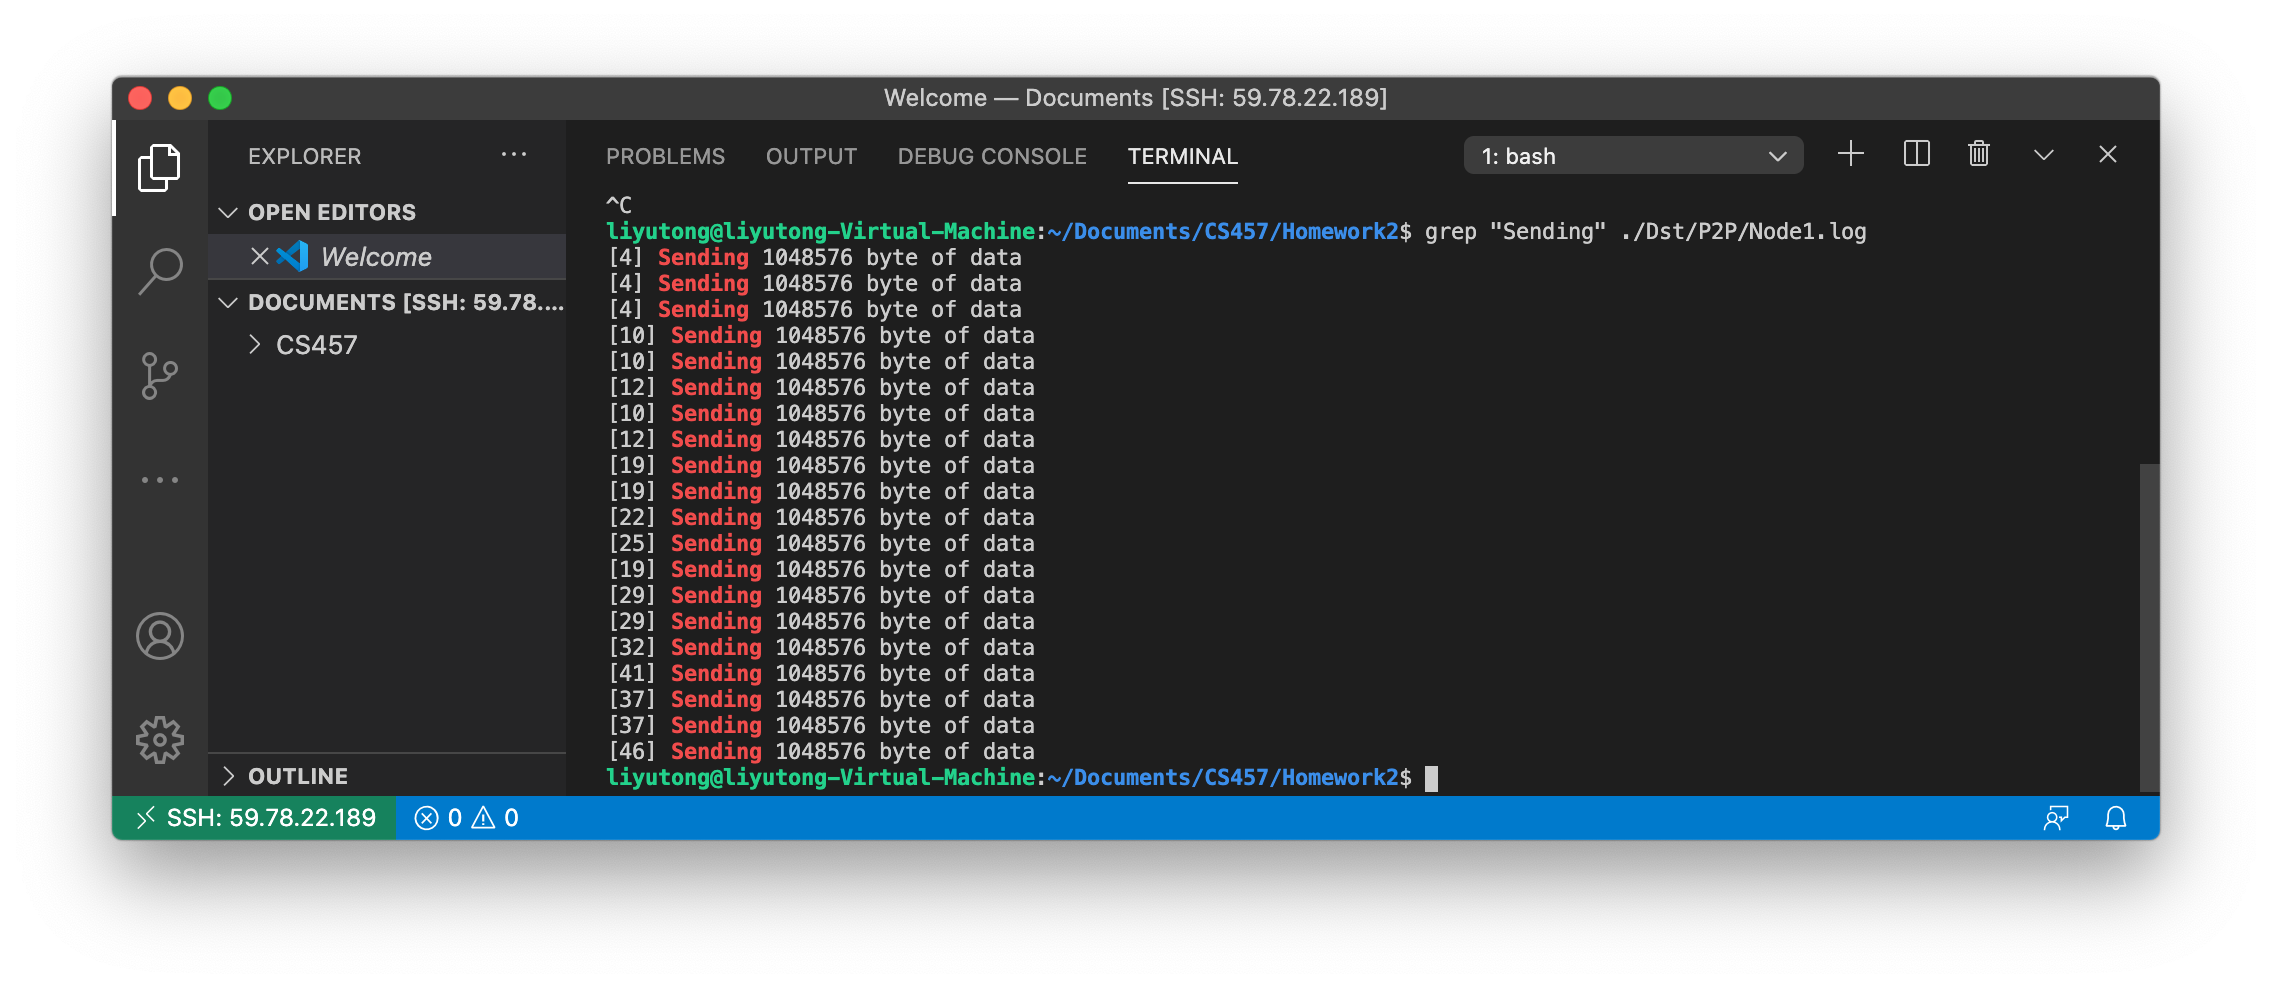
\includegraphics[scale=0.35]{img/upload}
	\caption{Node1 upload detail, $\mathtt{Number \ Client} = 5$}
	\label{upload}
\end{figure}
The Node1 only uploaded 20MiB of file. Its upload overhead is greatly reduced.